\subsubsection{\Destruction}\label{ssec:designdims:destruction} 

\begin{figure}[t]
  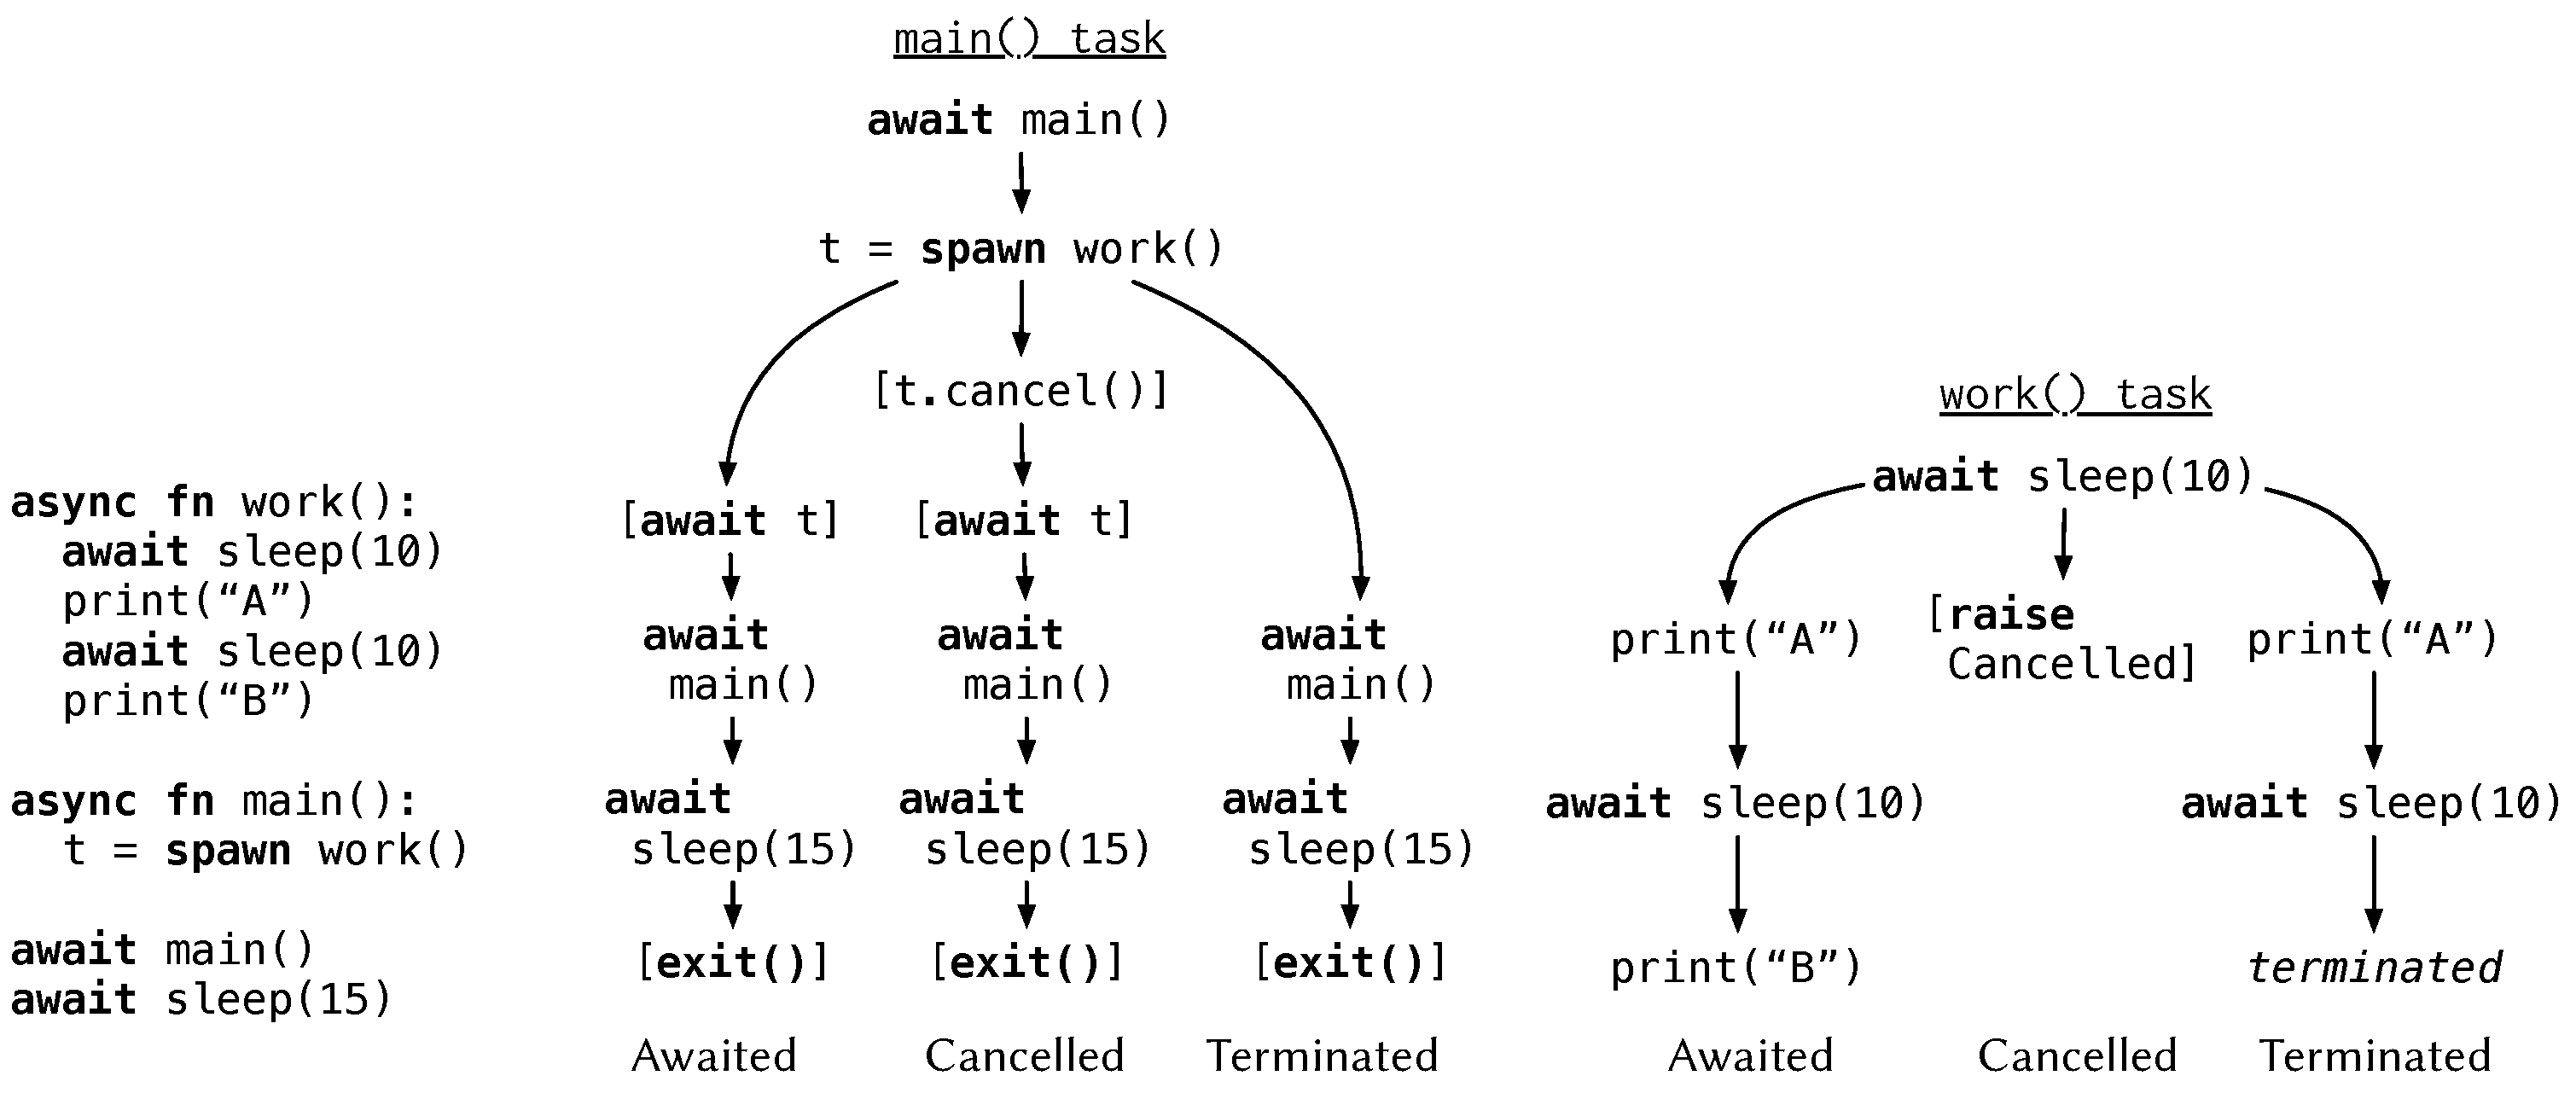
\includegraphics[width=\linewidth]{f/destruction.pdf}
  \caption{\Destruction [CAPTION TODO]}
  \label{fig:destruction}
\end{figure}


Once a language has decided that it is time to destruct a task, we encounter yet another point of divergence: what does it mean to destruct a task? For example, consider the program in \Cref{fig:destruction}. At the end of the \extent of the spawned \lstinline[language=Pseudo]|work()| task (either end of \lstinline[language=Pseudo]|main()| for \dyn \extent, or end of program for \indef \extent), what happens to the \lstinline[language=Pseudo]|work()| task? Today's languages offer three possibilities: to \emph{await} the task, to \emph{cancel} the task, and to \emph{terminate} the task.

The \destruction dimension is orthogonal to \extent. \Js is a language with \indef \extent and awaiting destruction --- \Cref{fig:extent} previously showed an example relying on this pair of design decisions. Python+Trio is a language/system with \dyn \extent and awaiting destruction, as tasks are tied to a ``nursery,'' and the nursery waits until all its child tasks are completed before exiting. The awaiting column in \Cref{fig:destruction} demonstrates Trio semantics, where the program would print ``ABC'' by waiting for the \lstinline[language=Pseudo]|work()| task to before exiting \lstinline[language=Pseudo]|main()|.

Most other designs opt to cancel tasks at the end of extent, such as Swift, Rust+Tokio, Rust+Smol, and Python+Asyncio. [TODO: ARE SMOL AND SWIFT ACTUALLY COMPARABLE?]


% The \Task Destruction axis defines what happens to a task when the \task object is destroyed by the system. The possible values are: \textit{awaited,} \textit{cancelled,} or \textit{terminated.}

% \Cref{fig:designdims:destruction:await} shows an example JavaScript program that awaits \tasks on destruction~\missingcite, even though there is no explicit \code{await} keyword. The program terminates after 10 seconds and prints ``exiting'' and ``done.''

% \Cref{fig:designdims:destruction:cancel} shows an example Swift program that cancels a running task on destruction~\missingcite. Because that task is executing a long sleep operation, the sleep is cancelled --- on cancellation \code{Task.sleep} raises an exception that we suppress with the \code{try?} keyword --- and the program continues executing. The program terminates after ~0.5 seconds and prints ``exiting,'' ``cancelled'' and ``done.''

% \Cref{fig:designdims:destruction:term} shows an example \CSharp program that terminates running \tasks on destruction~\missingcite. The program terminates after ~0.5 seconds and prints ``exiting.''

% Where your language falls on the destruction axis informs the safety and responsiveness of the system. Await destruction allows running \tasks to complete, which provides data/invariant integrity for the program at the expense of responsiveness.

% Cancel destruction may provide \tasks the chance to safely reclaim resources --- depending on the language's chosen cancellation semantics --- however, programs may still suffer from responsiveness issues if cancelling a \task requires the \task's cooperation. We discuss cancellation semantics in \Cref{ssec:designdims:cancellation}.

% Terminate destruction prioritizes speed over safety. A running \task may hold system resources or be in the middle of an operation, by cancelling the \task the system risks deadlocks and breaking logical invariants.
